\documentclass[10pt,twocolumn,letterpaper]{article}

\usepackage{cvpr}
\usepackage{times}
\usepackage{epsfig}
\usepackage{graphicx}
\usepackage{amsmath}
\usepackage{amssymb}
\usepackage{algorithm,algorithmicx,algpseudocode}
\usepackage{subfig}

\newcommand{\rulesep}{\unskip\ \vrule\ }


% Include other packages here, before hyperref.

% If you comment hyperref and then uncomment it, you should delete
% egpaper.aux before re-running latex.  (Or just hit 'q' on the first latex
% run, let it finish, and you should be clear).
\usepackage[breaklinks=true,bookmarks=false]{hyperref}

\cvprfinalcopy % *** Uncomment this line for the final submission

\def\cvprPaperID{****} % *** Enter the CVPR Paper ID here
\def\httilde{\mbox{\tt\raisebox{-.5ex}{\symbol{126}}}}

% Pages are numbered in submission mode, and unnumbered in camera-ready
%\ifcvprfinal\pagestyle{empty}\fi
\setcounter{page}{4321}
\begin{document}

%%%%%%%%% TITLE
\title{Investigating Model-Agnostic Meta-Learning for Fast Adaptation of Deep Networks}

\author{Mayank Agarwal\\
University of Massachusetts Amherst\\
{\tt\small mayankagarwa@cs.umass.edu}
}

\maketitle
%\thispagestyle{empty}

%%%%%%%%% ABSTRACT
\begin{abstract}
   The goal of this project is to implement the Model-Agnostic Meta-Learning (MAML) algorithm introduced by Chelsea Finn et. al. in    \cite{finn2017model}, and investigate the effect MAML has on the features learned by the network. MAML is a meta-learning technique that trains a network on a variety of different tasks, such that it can solve a new task using only a small number of training samples. Unlike standard parameter update schemes like SGD, etc., MAML explicitly trains the network such that it can be easily adapted to a new task with few samples. MAML is a generic algorithm which can be applied to supervised, unsupervised, and reinforcement learning, and has been shown to achieve state-of-the-art performances on certain classification tasks and good performance on other tasks. 
\end{abstract}

%%%%%%%%% BODY TEXT
\section{Introduction}

Deep learning methods have shown great success in fields such as Computer Vision and Natural Language understanding - even achieving "super-human" performance in certain fields. However, contemporary deep learning models require huge amounts of data to train, failing which they run the risk of over-fitting and not generalizing well on unseen data. This is in direct contrast to the natural way of learning where a human can learn and generalize about a subject after seeing only a few examples. This notion of learning is called "few-shot learning", where the aim is to train a model using only a few training samples.

Meta-Learning, or learning to learn new tasks quickly, dates back to the late 1980s and early 1990s, but there has been a resurgence in meta-learning to solve the task of few-shot learning. Recent meta-learning techniques typically fall in one of the following three categories: 1) Recurrent models, where a recurrent network, eg an LSTM, is trained to take in data sequentially and then process new inputs from the task, 2) Metric learning, which learns an efficient and effective comparison scheme to compare between the training data and the new input data, and 3) Learning optimizers, where one network (meta-learner) learns how to update the learner network such that it can effectively learn a new task.

MAML, on the other hand, aims to learn an initialization of the network that allows it to adapt to new tasks with only a few training samples. According to the authors, MAML can be seen from a feature learning standpoint as learning an internal representation that is broadly suited for many tasks. 

This project aims to learn more about the features MAML learns, and aims to understand the difference between the features learned by a network trained using MAML and standard training procedures independently.

%-------------------------------------------------------------------------

\section{Problem statement}

\subsection{Model-Agnostic Meta-Learning}

Model-Agnostic Meta-Learning aims to learn the parameters of any standard model in such a way as to allow the model to quickly adapt to new tasks. MAML performs a one-step lookahead of the parameters through gradient descent, and finally updates the parameters to minimize the loss on future tasks. The algorithm is describe in \ref{algo}. This procedure is generic and is applicable to any gradient descent based learning method. I intend to apply this to supervised classification problem and investigate the features applicable to this particular domain.

\begin{algorithm}
  \caption{MAML for few-shot supervised learning}
  \label{algo}
  \begin{algorithmic}[1]
  \Require $p(T)$: distribution over tasks
  \Require $\alpha, \beta$: step size hyperparameters
  
  \State randomly initialize $\theta$
  \While{not done}
	\State Sample batch of tasks $T_i \sim p(T_i)$  
	
	\For{all $T_i$}
	
	\State Sample K datapoints $D = \{x^{(j)}, y^{(j)}\}$ from $T_i$
	\State Evaluate $\nabla_\theta L_{T_i}(f_\theta)$ using $D$ and $L_{T_i}$
	
	\State Compute adapted parameters with gradient descent:
	$\theta_i^{'} = \theta - \alpha \nabla_{\theta} L_{T_i} (f_\theta)$
	
	\State Sample datapoints $D_i^{'} = \{x^{(j)}, y^{(j)}\}$  from $T_i$ for the meta-update
	
	\EndFor
	
	\State Update $\theta \leftarrow \theta - \beta \nabla_\theta \sum_{T_i \sim p(T_i)} L_{T_i}(f_{\theta^{'}})$ using each $D_i^{'}$ and $L_{T_i}$
  
  \EndWhile
  \end{algorithmic}
\end{algorithm}

\subsection{Feature visualization}

Understanding the differences between features learned by a model trained with and without MAML would require visualizing different aspects of the network. These would include both feature visualization as well as attribution studies. Visualization techniques would include optimizing an image to maximize certain objective, finding dataset examples that maximally or minimally activate a neuron, class saliency maps, and others. \cite{olah2017feature}

\subsection{Dataset}

Since this is a few-shot learning domain, I'll be using datasets that provide only a few examples of each class. In addition to using curated datasets, I will also be creating appropriate datasets from more conventional datasets.

For curated datasets, I'll be using the Omniglot dataset \cite{lake2015human}. Omniglot dataset contains 20 training samples each of 1623 different handwritten characters. These characters come from 50 different alphabets. Each of these training samples is drawn by a different person.

Besides Omniglot, I will also be creating few-shot learning datasets from MNIST and CIFAR-10, by randomly selecting K examples from each class for training, test, and validation data.


\section{Preliminary Results}

\subsection{Baseline Model}

A fully-connected network with [256, 128, 64, 64, 10] neurons in each successive layer is prepared. After each layer is a Batch Normalization layer and then a ReLU layer. This model is trained on the complete MNIST data and its features visualized to act as a reference for the features generated in a standard classification task.

This model is trained for 5 epochs with mini-batches of size 256. Adam optimizer is used with initial learning rate 0.001, beta1 and beta2 set to 0.9 and 0.999 respectively. Additionally, L2 regularization with regularization strength of 0.01 is used.

The model achieves a test accuracy of 96.71\%. The loss curve and the training-validation accuracy over epochs is shown in \ref{fig:loss}

\begin{figure}%
	\centering
	\subfloat{{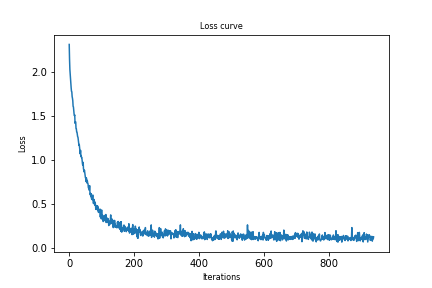
\includegraphics[scale=0.3]{images/1-fc-mnist/loss_curve} }}%
    %\qquad
    \subfloat{{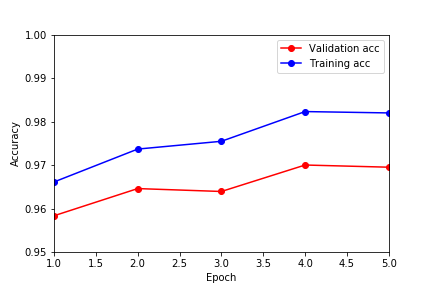
\includegraphics[scale=0.3]{images/1-fc-mnist/train_val_acc} }}%
    
    \caption{Loss curve and Train-val accuracy}
	\label{fig:loss}
\end{figure}


\subsection{Baseline Visualizations}

\subsubsection{First layer filter visualization}

The first affine layer of the model consists of 256 neurons and the weights of this layer are of the dimension [784, 256]. Thus, each neuron weight can be visualized to produce 256 neuron visualizations. Some manually picked visualization are shown in \ref{fig:fc1-filtervis}. Some of these neurons have aligned themselves to learn specific character patterns like the shape of 5, and the common shapes of 3 and 8.


\begin{figure}%
    \centering
    \subfloat{{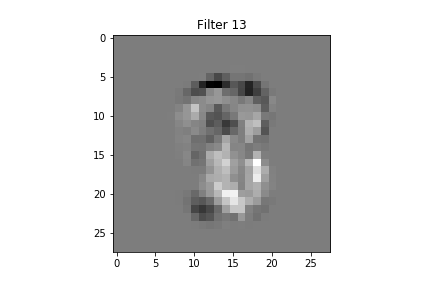
\includegraphics[width=3cm]{images/1-fc-mnist/filter-13} }}%
    %\qquad
    \subfloat{{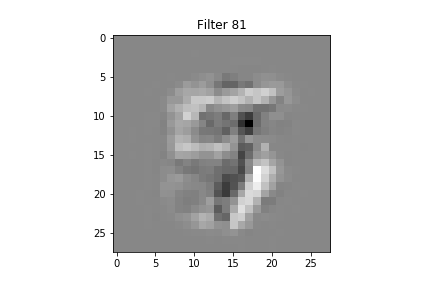
\includegraphics[width=3cm]{images/1-fc-mnist/filter-81} }}%
%    \qquad
    \subfloat{{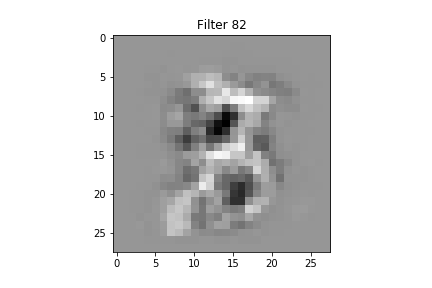
\includegraphics[width=3cm]{images/1-fc-mnist/filter-82} }}%
    \\    
    \centering
    
    \subfloat{{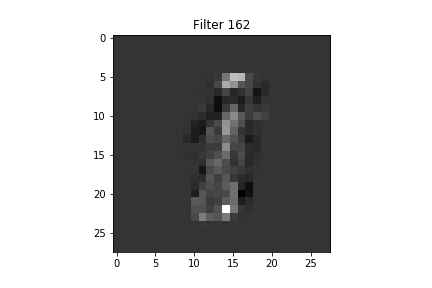
\includegraphics[width=3cm]{images/1-fc-mnist/filter-162} }}%
    %\qquad
    \subfloat{{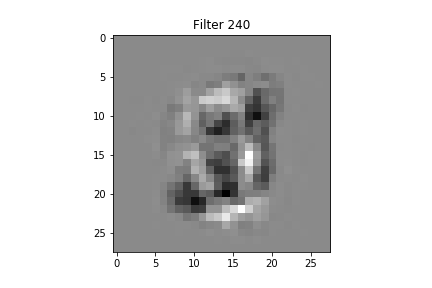
\includegraphics[width=3cm]{images/1-fc-mnist/filter-240} }}%
%    \qquad
    \subfloat{{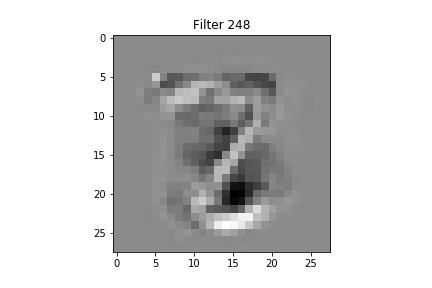
\includegraphics[width=3cm]{images/1-fc-mnist/filter-248} }}%
    \caption{First layer filters visualized}%
    \label{fig:fc1-filtervis}%
\end{figure}


\subsubsection{Visualize the final affine layer}

The layers in a neural network learn features of the input data which is then fed to the affine layer with softmax for classification. The final affine layer feeding into the classification layer can be understood to have learned representation that is easily classifiable.

Test data is fed through the network and the final affine layer outputs are collected for each test data sample. These encodings are in 64 dimensions and therefore need to reduced in dimensions. Using t-SNE \cite{maaten2008visualizing} and PCA \cite{wold1987principal}, I reduce the dimensions to 2, plotted these points and then color-coded them according to their label. t-SNE visualization is shown in \ref{fig:tsne}, and PCA visualization is shown in \ref{fig:pca}. As can been in the t-SNE visualization, the output of the final affine layer is clustered according the label.


\begin{figure}%
\centering
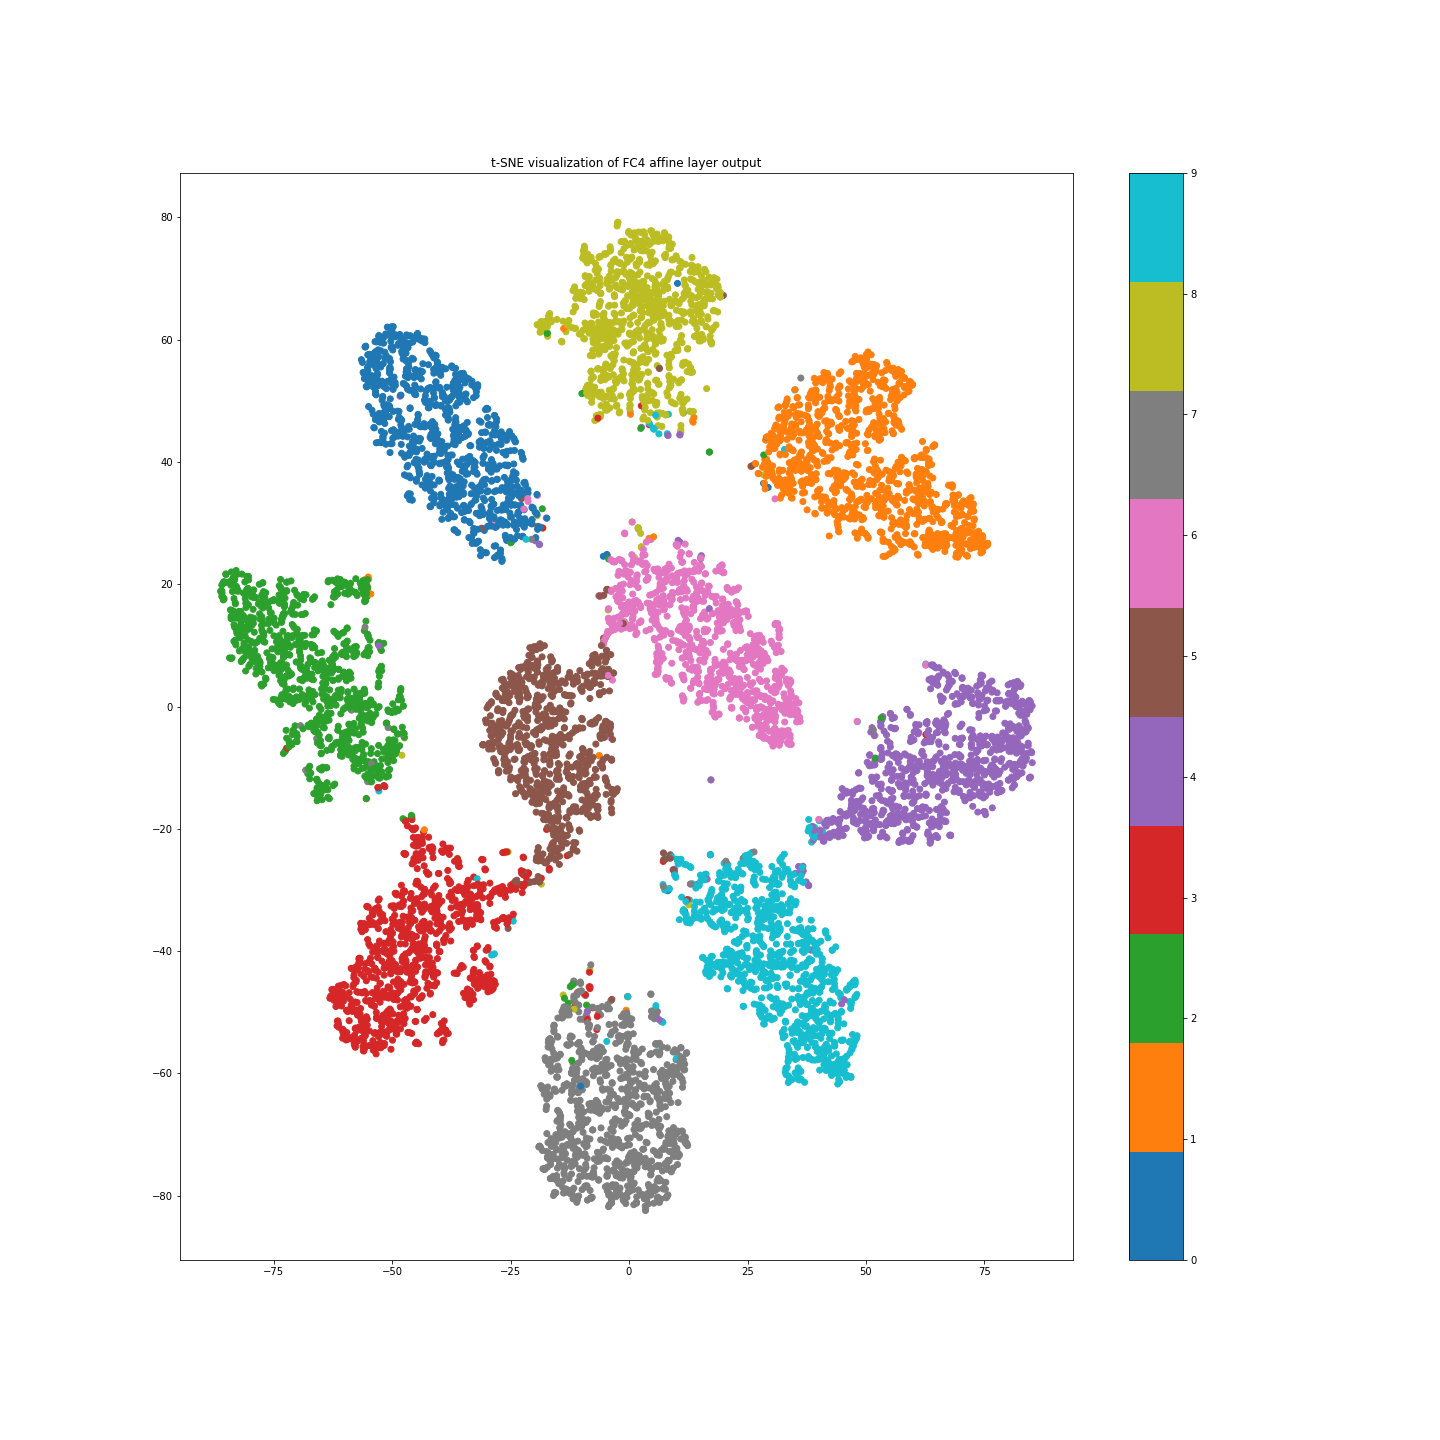
\includegraphics[scale=0.15]{images/1-fc-mnist/tsne_fc4_output}
\caption{t-SNE visualization of the final affine layer}
\label{fig:tsne}
\end{figure}

\begin{figure}%
\centering
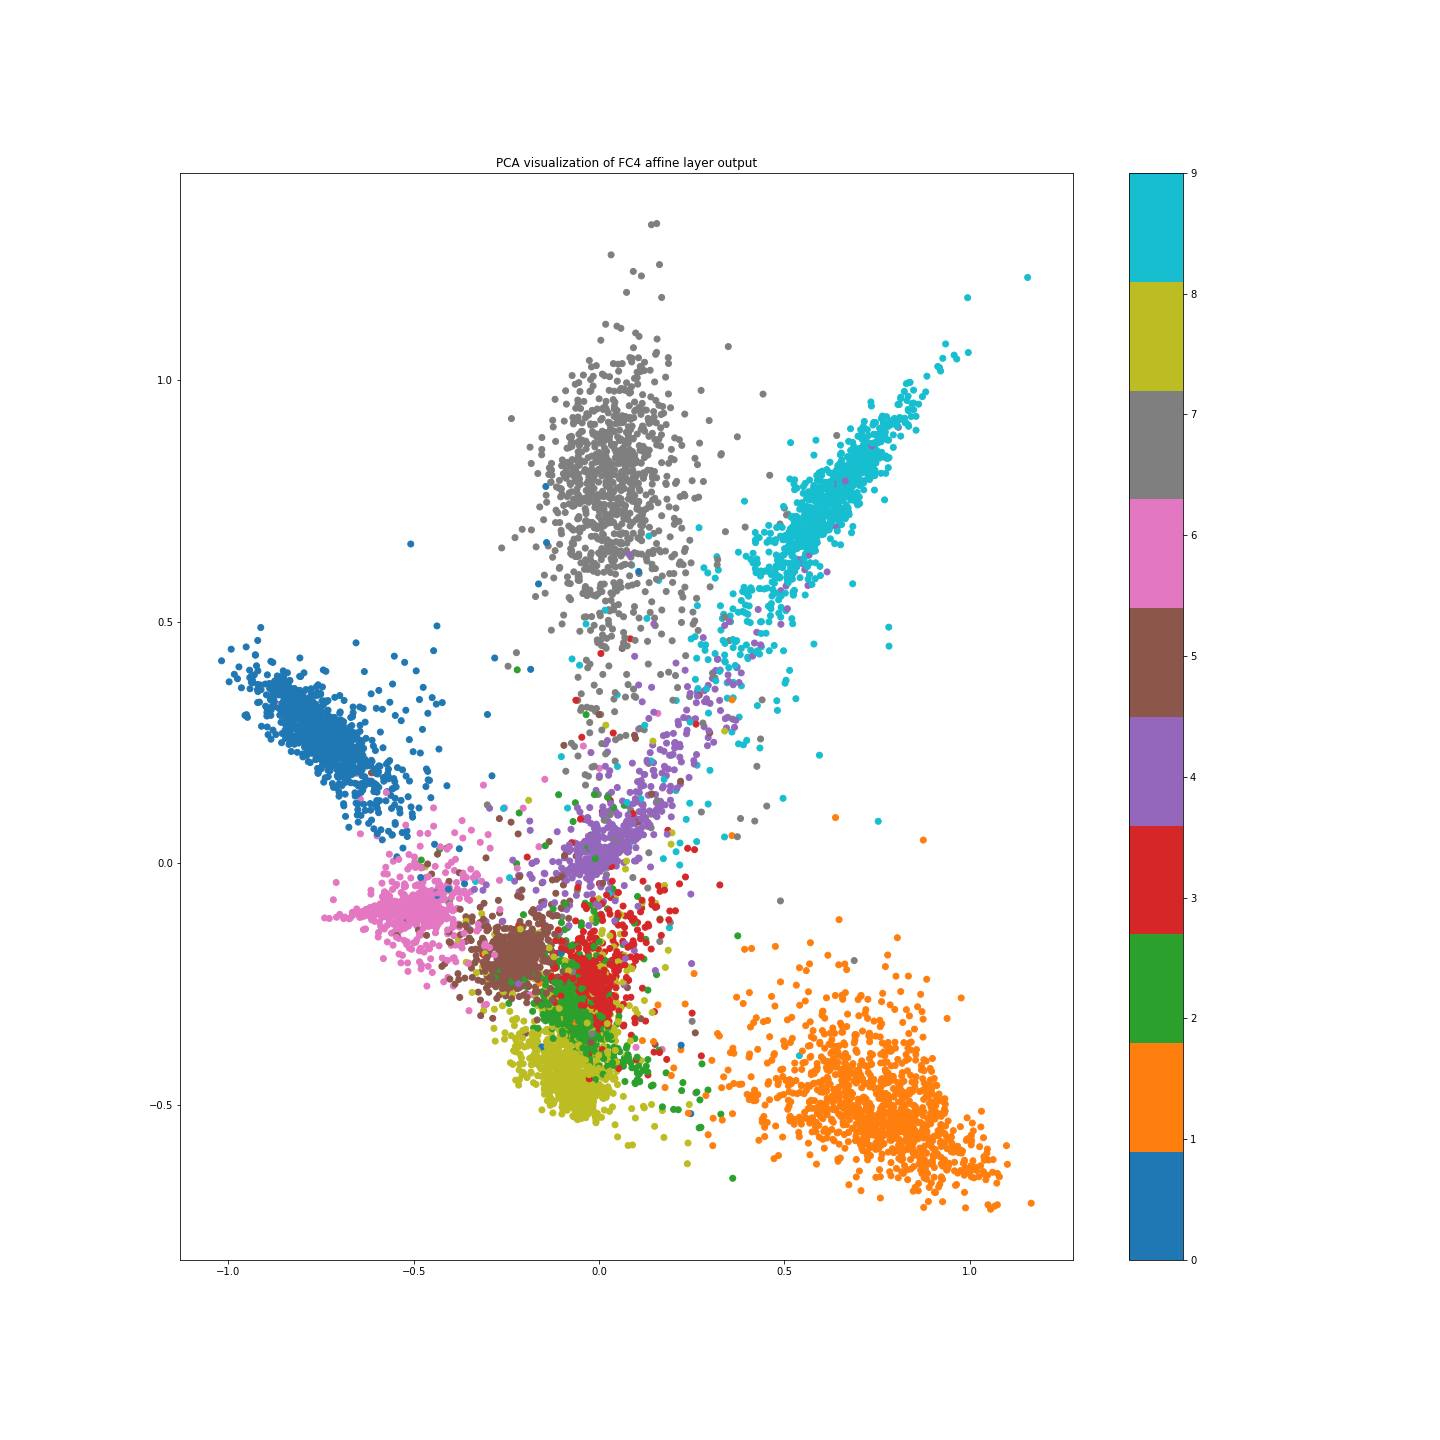
\includegraphics[scale=0.15]{images/1-fc-mnist/pca_fc4_output}
\caption{PCA visualization of the final affine layer}
\label{fig:pca}
\end{figure}


\subsubsection{Neuron activations}

Neuron activation with certain data samples can be used to determine the preference of certain neurons in arbitrary layers of the network. 

Here, I feed test data through the trained network, and record the activations for neurons in the third and fourth Batch normalization \cite{ioffe2015batch} layer. Studying the examples (shown in \ref{fig:neuron-vis}) which maximally and minimally activate neurons in these layers indicate the affinity and aversion of these neurons.

\begin{figure}%
    \centering
    \text{BN4/N9}
    \subfloat{{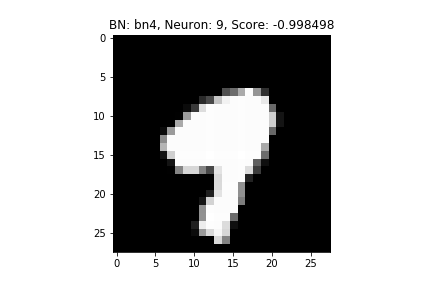
\includegraphics[width=1cm]{images/1-fc-mnist/bn4/9/min/2} }}%
    \subfloat{{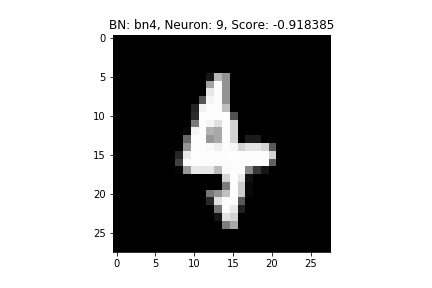
\includegraphics[width=1cm]{images/1-fc-mnist/bn4/9/min/1} }}%
    \subfloat{{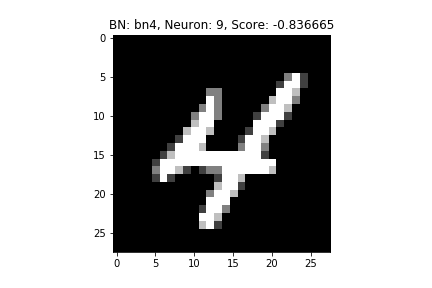
\includegraphics[width=1cm]{images/1-fc-mnist/bn4/9/min/0} }}%
    \rulesep
    \subfloat{{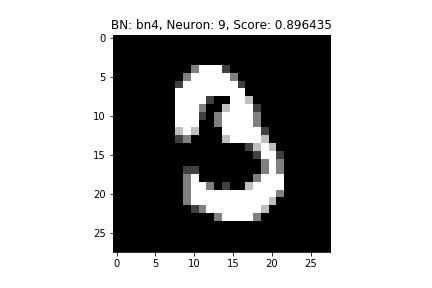
\includegraphics[width=1cm]{images/1-fc-mnist/bn4/9/max/0} }}%
    \subfloat{{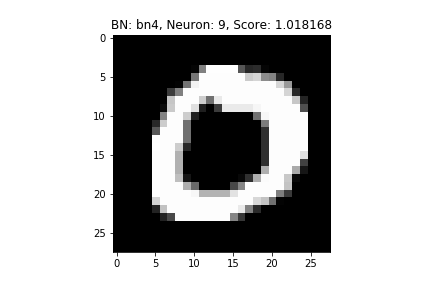
\includegraphics[width=1cm]{images/1-fc-mnist/bn4/9/max/1} }}%
    \subfloat{{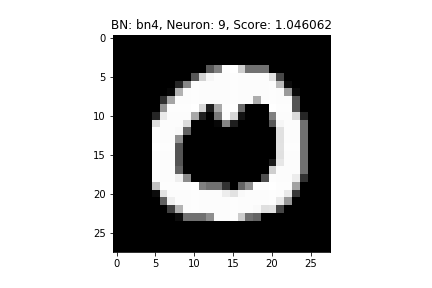
\includegraphics[width=1cm]{images/1-fc-mnist/bn4/9/max/2} }}%
    \\
    \text{BN4/N226}
    \subfloat{{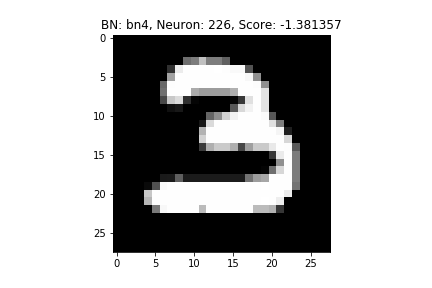
\includegraphics[width=1cm]{images/1-fc-mnist/bn4/226/min/2} }}%
    \subfloat{{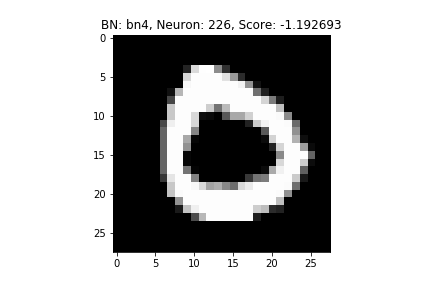
\includegraphics[width=1cm]{images/1-fc-mnist/bn4/226/min/1} }}%
    \subfloat{{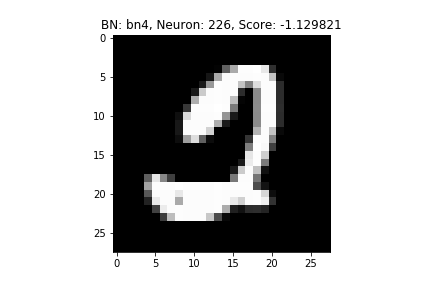
\includegraphics[width=1cm]{images/1-fc-mnist/bn4/226/min/0} }}%
    \rulesep
    \subfloat{{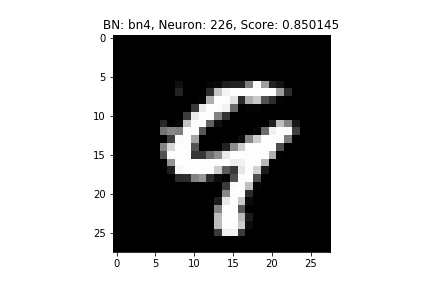
\includegraphics[width=1cm]{images/1-fc-mnist/bn4/226/max/0} }}%
    \subfloat{{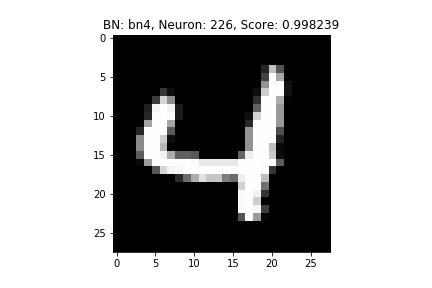
\includegraphics[width=1cm]{images/1-fc-mnist/bn4/226/max/1} }}%
    \subfloat{{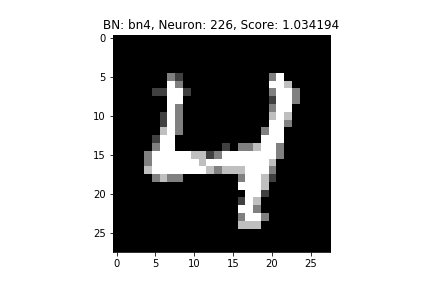
\includegraphics[width=1cm]{images/1-fc-mnist/bn4/226/max/2} }}%
    \\
    \text{BN3/N210}
    \subfloat{{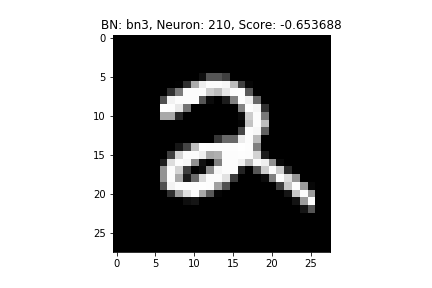
\includegraphics[width=1cm]{images/1-fc-mnist/bn3/210/min/2} }}%
    \subfloat{{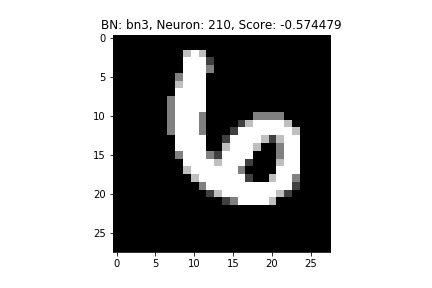
\includegraphics[width=1cm]{images/1-fc-mnist/bn3/210/min/1} }}%
    \subfloat{{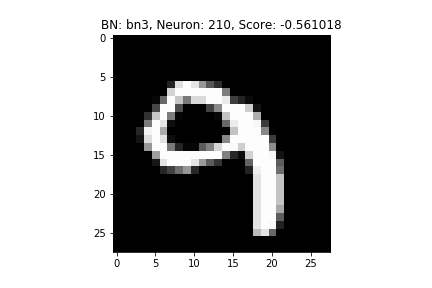
\includegraphics[width=1cm]{images/1-fc-mnist/bn3/210/min/0} }}%
    \rulesep
    \subfloat{{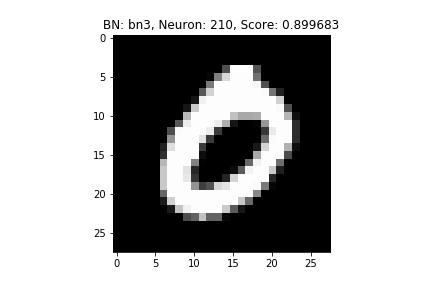
\includegraphics[width=1cm]{images/1-fc-mnist/bn3/210/max/0} }}%
    \subfloat{{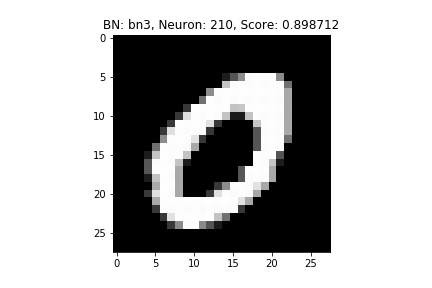
\includegraphics[width=1cm]{images/1-fc-mnist/bn3/210/max/1} }}%
    \subfloat{{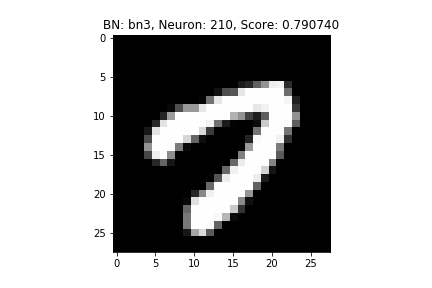
\includegraphics[width=1cm]{images/1-fc-mnist/bn3/210/max/2} }}%
    
    \caption{Examples that minimally (left) and Maximally (right) activate a neuron in Batch norm layer BN[X] and Neuron N[Y]}%
    \label{fig:neuron-vis}%
\end{figure}




\section{Current and Future work}

The MAML parameter update equation involves one-step lookahead. This requires computing a Hessian-vector product. Currently, I am working on deriving the parameter update equation involving Hessian matrices, and also a first-order approximation of it. The parameter update equations is derived to be:

\begin{equation}
\theta \leftarrow \theta - \beta \sum_{T_i \sim p(T)} \Big[ \frac{\partial}{\partial \theta_i^{'}} L_{T_i} (f_{\theta^{'}}) - \alpha \frac{\partial}{\partial \theta_i^{'}} L_{T_i} (f_{\theta^{'}}) \frac{\partial^2}{\partial \theta \partial \theta^T} L_{T_i} (f_{\theta_i}) \Big]
\end{equation}


Hessian-vector product used above can be approximated as:

\begin{equation}
\frac{\partial}{\partial \theta_i^{'}} L_{T_i} (f_{\theta^{'}}) \frac{\partial^2}{\partial \theta \partial \theta^T} L_{T_i} (f_{\theta_i}) = \frac{\nabla_{\theta_i} f_{\theta_i + \epsilon \nabla_{\theta_i^{'}} L(f_{\theta_i^{'}})} - \nabla_{\theta_i} f_{\theta_i - \epsilon \nabla_{\theta_i^{'}} L(f_{\theta_i^{'}})}}{2\epsilon}
\end{equation}

Next steps in the project would be to implement MAML with the aforementioned update equations in PyTorch, train a model with MAML, visualize its features and compare.
%-------------------------------------------------------------------------

{\small
\bibliographystyle{ieee}
\bibliography{egbib}
}

\end{document}
